\section{Date: 2026-10-23}
\noindent \textbf{Series ID: STTMINWGDC} 

\noindent This series is titled State Minimum Wage Rate for District of Columbia and has a frequency of Annual. The units are Dollars per Hour and the seasonal adjustment is Not Seasonally Adjusted.The observation start date is 1968-01-01 and the observation end date is 2026-01-01.The popularity of this series is 21. \\ 

\noindent \textbf{Series ID: ATNHPIUS37900Q} 

\noindent This series is titled All-Transactions House Price Index for Peoria, IL (MSA) and has a frequency of Quarterly. The units are Index 1995:Q1=100 and the seasonal adjustment is Not Seasonally Adjusted.The observation start date is 1979-04-01 and the observation end date is 2026-04-01.The popularity of this series is 2. \\ 

\subsection{Raw Regression}
\noindent Regresses the two series against each other directly. A significant result here can come just as easily from both series sharing a long-run trend as from any real relationship.

\begin{center}
\begin{tabular}{lclc}
\toprule
\textbf{Dep. Variable:}          & value\_fred\_ATNHPIUS37900Q & \textbf{  R-squared:         } &     0.773   \\
\textbf{Model:}                  &             OLS             & \textbf{  Adj. R-squared:    } &     0.768   \\
\textbf{Method:}                 &        Least Squares        & \textbf{  F-statistic:       } &     153.3   \\
\textbf{Date:}                   &       Fri, 23 Oct 2026      & \textbf{  Prob (F-statistic):} &  4.28e-16   \\
\textbf{Time:}                   &           15:59:09          & \textbf{  Log-Likelihood:    } &   -215.63   \\
\textbf{No. Observations:}       &                47           & \textbf{  AIC:               } &     435.3   \\
\textbf{Df Residuals:}           &                45           & \textbf{  BIC:               } &     439.0   \\
\textbf{Df Model:}               &                 1           & \textbf{                     } &             \\
\textbf{Covariance Type:}        &          nonrobust          & \textbf{                     } &             \\
\bottomrule
\end{tabular}
\begin{tabular}{lcccccc}
                                 & \textbf{coef} & \textbf{std err} & \textbf{t} & \textbf{P$> |$t$|$} & \textbf{[0.025} & \textbf{0.975]}  \\
\midrule
\textbf{const}                   &      51.3736  &        7.417     &     6.926  &         0.000        &       36.434    &       66.313     \\
\textbf{value\_fred\_STTMINWGDC} &      10.0257  &        0.810     &    12.383  &         0.000        &        8.395    &       11.656     \\
\bottomrule
\end{tabular}
\begin{tabular}{lclc}
\textbf{Omnibus:}       & 16.895 & \textbf{  Durbin-Watson:     } &    0.093  \\
\textbf{Prob(Omnibus):} &  0.000 & \textbf{  Jarque-Bera (JB):  } &    3.651  \\
\textbf{Skew:}          &  0.192 & \textbf{  Prob(JB):          } &    0.161  \\
\textbf{Kurtosis:}      &  1.690 & \textbf{  Cond. No.          } &     19.3  \\
\bottomrule
\end{tabular}
%\caption{OLS Regression Results}
\end{center}

Notes: \newline
 [1] Standard Errors assume that the covariance matrix of the errors is correctly specified.

\begin{figure}
\centering
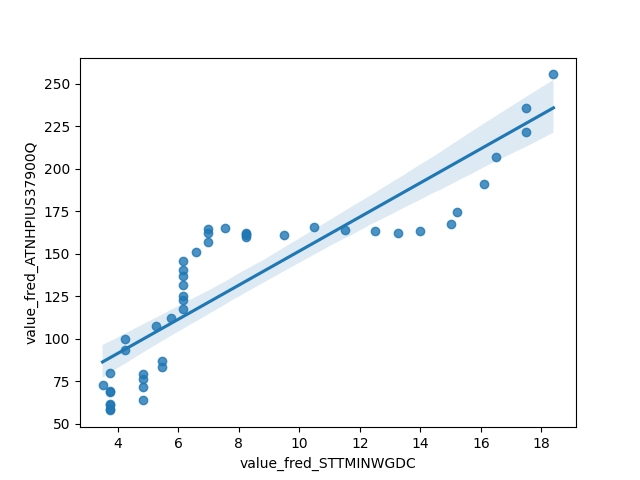
\includegraphics[scale = 0.9]{plots/plot_2026-10-23.png}
\caption{Raw Regression Plot for 2026-10-23}
\end{figure}
\newpage
\subsection{Detrended Regression}
\noindent Regresses the residuals of each series after removing its own linear time trend, so a shared trend can no longer drive the result on its own. A relationship that stays significant here is better evidence of a genuine link between the two series.

\begin{center}
\begin{tabular}{lclc}
\toprule
\textbf{Dep. Variable:}                     & value\_fred\_ATNHPIUS37900Q\_detrended & \textbf{  R-squared:         } &     0.000   \\
\textbf{Model:}                             &                  OLS                   & \textbf{  Adj. R-squared:    } &    -0.022   \\
\textbf{Method:}                            &             Least Squares              & \textbf{  F-statistic:       } &   0.01385   \\
\textbf{Date:}                              &            Fri, 23 Oct 2026            & \textbf{  Prob (F-statistic):} &    0.907    \\
\textbf{Time:}                              &                15:59:09                & \textbf{  Log-Likelihood:    } &   -191.61   \\
\textbf{No. Observations:}                  &                     47                 & \textbf{  AIC:               } &     387.2   \\
\textbf{Df Residuals:}                      &                     45                 & \textbf{  BIC:               } &     390.9   \\
\textbf{Df Model:}                          &                      1                 & \textbf{                     } &             \\
\textbf{Covariance Type:}                   &               nonrobust                & \textbf{                     } &             \\
\bottomrule
\end{tabular}
\begin{tabular}{lcccccc}
                                            & \textbf{coef} & \textbf{std err} & \textbf{t} & \textbf{P$> |$t$|$} & \textbf{[0.025} & \textbf{0.975]}  \\
\midrule
\textbf{const}                              &     1.51e-14  &        2.127     &   7.1e-15  &         1.000        &       -4.283    &        4.283     \\
\textbf{value\_fred\_STTMINWGDC\_detrended} &       0.1420  &        1.207     &     0.118  &         0.907        &       -2.288    &        2.572     \\
\bottomrule
\end{tabular}
\begin{tabular}{lclc}
\textbf{Omnibus:}       &  1.830 & \textbf{  Durbin-Watson:     } &    0.176  \\
\textbf{Prob(Omnibus):} &  0.400 & \textbf{  Jarque-Bera (JB):  } &    1.367  \\
\textbf{Skew:}          &  0.418 & \textbf{  Prob(JB):          } &    0.505  \\
\textbf{Kurtosis:}      &  3.012 & \textbf{  Cond. No.          } &     1.76  \\
\bottomrule
\end{tabular}
%\caption{OLS Regression Results}
\end{center}

Notes: \newline
 [1] Standard Errors assume that the covariance matrix of the errors is correctly specified.

\begin{figure}
\centering
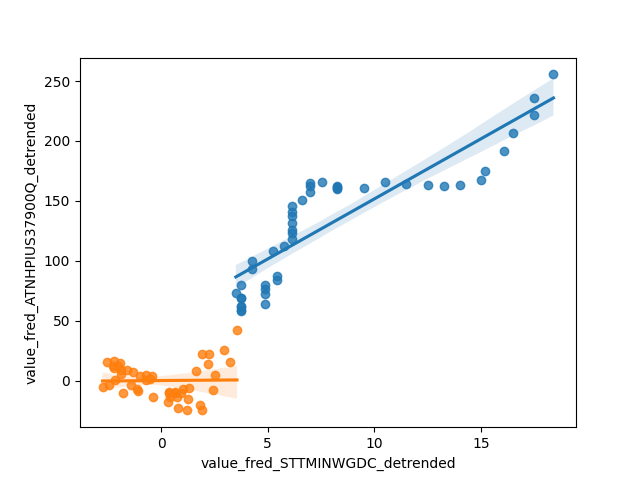
\includegraphics[scale = 0.9]{plots/plot_2026-10-23_detrended.png}
\caption{Detrended Regression Plot for 2026-10-23}
\end{figure}
\newpage
